\documentclass[conference]{IEEEtran}
\IEEEoverridecommandlockouts

\usepackage{cite}
\usepackage{amsmath,amssymb,amsfonts}
\usepackage{algorithmic}
\usepackage{graphicx}
\usepackage{textcomp}
\usepackage{xcolor}
\usepackage{booktabs}
\usepackage{hyperref}
\usepackage{siunitx}
\graphicspath{{../../}{./}{results/figures/}{figures/}}

% Paper numbers — auto-generated, do not edit by hand
\IfFileExists{paper_numbers.tex}{% Auto-generated by src/final.py — DO NOT EDIT BY HAND
% All numbers derived from results/scores/*.npy
\newcommand{\BaseRateTest}{0.1317\%}
\newcommand{\BaseRateVal}{0.1001\%}
\newcommand{\NTest}{56{,}962}
\newcommand{\NVal}{56{,}961}
\newcommand{\NFraudTest}{75}
\newcommand{\NFraudVal}{57}
\newcommand{\PRAUCTestPCA}{0.7425}
\newcommand{\PRAUCValPCA}{0.7066}
\newcommand{\RecallFPRHalfPctPCA}{0.7733}
\newcommand{\PrecCapHalfPctPCA}{0.2000}
\newcommand{\PRAUCTestLOF}{0.4478}
\newcommand{\PRAUCValLOF}{0.4069}
\newcommand{\RecallFPRHalfPctLOF}{0.7200}
\newcommand{\PrecCapHalfPctLOF}{0.1860}
\newcommand{\PRAUCTestGMM}{0.4142}
\newcommand{\PRAUCValGMM}{0.1950}
\newcommand{\RecallFPRHalfPctGMM}{0.6933}
\newcommand{\PrecCapHalfPctGMM}{0.1825}
\newcommand{\PRAUCTestOCSVM}{0.1322}
\newcommand{\PRAUCValOCSVM}{0.0613}
\newcommand{\RecallFPRHalfPctOCSVM}{0.6933}
\newcommand{\PrecCapHalfPctOCSVM}{0.1649}
\newcommand{\PRAUCTestIFOREST}{0.0577}
\newcommand{\PRAUCValIFOREST}{0.0330}
\newcommand{\RecallFPRHalfPctIFOREST}{0.3467}
\newcommand{\PrecCapHalfPctIFOREST}{0.0772}
}{% --- Paper Numbers (Inlined) ---
% Auto-generated by src/final.py — DO NOT EDIT BY HAND
% All numbers derived from results/scores/*.npy
\newcommand{\BaseRateTest}{0.1317\%}
\newcommand{\BaseRateVal}{0.1001\%}
\newcommand{\NTest}{56{,}962}
\newcommand{\NVal}{56{,}961}
\newcommand{\NFraudTest}{75}
\newcommand{\NFraudVal}{57}
\newcommand{\PRAUCTestPCA}{0.7425}
\newcommand{\PRAUCValPCA}{0.7066}
\newcommand{\RecallFPRHalfPctPCA}{0.7733}
\newcommand{\PrecCapHalfPctPCA}{0.2000}
\newcommand{\PRAUCTestLOF}{0.4478}
\newcommand{\PRAUCValLOF}{0.4069}
\newcommand{\RecallFPRHalfPctLOF}{0.7200}
\newcommand{\PrecCapHalfPctLOF}{0.1860}
\newcommand{\PRAUCTestGMM}{0.4142}
\newcommand{\PRAUCValGMM}{0.1950}
\newcommand{\RecallFPRHalfPctGMM}{0.6933}
\newcommand{\PrecCapHalfPctGMM}{0.1825}
\newcommand{\PRAUCTestOCSVM}{0.1322}
\newcommand{\PRAUCValOCSVM}{0.0613}
\newcommand{\RecallFPRHalfPctOCSVM}{0.6933}
\newcommand{\PrecCapHalfPctOCSVM}{0.1649}
\newcommand{\PRAUCTestIFOREST}{0.0577}
\newcommand{\PRAUCValIFOREST}{0.0330}
\newcommand{\RecallFPRHalfPctIFOREST}{0.3467}
\newcommand{\PrecCapHalfPctIFOREST}{0.0772}}

\def\BibTeX{{\rm B\kern-.05em{\sc i\kern-.025em b}\kern-.08em
    T\kern-.1667em\lower.7ex\hbox{E}\kern-.125emX}}

\begin{document}

\title{Card Fraud Triage via Gaussian Mixture Density Scoring:\\
Phase 1 — Machine Learning Evaluation\\
{\footnotesize Team T033, Section A, Project 26 — Rishihood University}}

\author{
\IEEEauthorblockN{Kushal Sarkar\textsuperscript{1},
                  Prachee Dhar\textsuperscript{2},
                  Apoorva Choudhary\textsuperscript{3},
                  Vani Rudra\textsuperscript{4},
                  Krishna Pramod Dubale\textsuperscript{5}}
\IEEEauthorblockA{Rishihood University, Sonipat, India\\
Enrollment: \textsuperscript{1}2401020033
            \textsuperscript{2}2401010330
            \textsuperscript{3}2401010092
            \textsuperscript{4}2401010490
            \textsuperscript{5}2401010239\\
Faculty: Shobhit Johri, Arun Chauhan, Ashwin Tewary}
}

\maketitle

\begin{abstract}
We frame credit card fraud detection as an unsupervised anomaly detection problem,
training models exclusively on legitimate transactions and scoring each transaction
by its deviation from the learned normal manifold.
We evaluate five methods on the ULB Credit Card Fraud dataset
(\NTest{} transactions, \NFraudTest{} test frauds, base rate \BaseRateTest{}):
Gaussian Mixture Model (GMM) density scoring, PCA reconstruction error,
Isolation Forest, One-Class SVM, and Local Outlier Factor.
PCA reconstruction error achieves the highest test PR-AUC (\PRAUCTestPCA{}),
catching \RecallFPRHalfPctPCA{} of test frauds at a 0.5\% false-positive
rate budget. GMM achieves PR-AUC \PRAUCTestGMM{} on test despite poor
validation performance, exposing instability under severe class imbalance.
We report precision-recall curves, recall at fixed FPR budgets, precision at
review capacity, bootstrap confidence intervals, and threshold analysis.
A future phase will compare a deep autoencoder reconstruction scorer.
\end{abstract}

\begin{IEEEkeywords}
anomaly detection, fraud detection, Gaussian mixture model, PCA reconstruction,
unsupervised learning, class imbalance, precision-recall
\end{IEEEkeywords}

%%% ─── 1. Introduction ────────────────────────────────────────────────────────
% === Inlined sections/p1_introduction ===
\section{Introduction}
\label{sec:introduction}

Financial transaction systems process billions of electronic operations daily under constant exposure to adversarial fraud syndicates \cite{leborgne2022handbook}. In retail banking, automated card fraud triage faces three severe operational constraints that violate standard supervised learning assumptions:
\begin{enumerate}
    \item \textbf{Extreme Class Imbalance:} Fraudulent events represent an ultra-rare class ($<0.2\%$). In the benchmark European credit card stream \cite{dalpozzolo2018credit}, only $492$ out of $284,807$ transactions ($0.1727\%$) are fraudulent. Trivial majority-class prediction yields $99.83\%$ accuracy while catching zero financial losses.
    \item \textbf{Verification Lag:} Ground-truth fraud labels are not available at transaction authorization time, emerging only days or weeks later following cardholder dispute resolutions \cite{carcillo2018scarff}.
    \item \textbf{Adversarial Non-Stationarity:} Fraud strategies evolve dynamically, while legitimate consumer spending undergoes circadian and seasonal shifts, creating ongoing distribution drift \cite{dalpozzolo2015calibrating}.
\end{enumerate}

To address label scarcity and delayed feedback, fraud triage can be formulated as an \emph{unsupervised anomaly detection} problem: models learn the probability density or bounding envelope of legitimate cardholder behavior, scoring unseen transactions by their deviation from normal patterns.

\subsection{Phase 1 Scope and Contributions}
In Phase~1 of Project T033, we evaluate classical machine learning and statistical density estimation methods for credit card fraud triage. We analyze Gaussian Mixture Models (GMM) estimated via Expectation-Maximization (EM) \cite{dempster1977maximum} alongside four classical baselines: PCA Reconstruction Error \cite{shyu2003novel}, Local Outlier Factor (LOF) \cite{breunig2000lof}, One-Class SVM (OC-SVM) \cite{scholkopf2001estimating}, and Isolation Forest \cite{liu2008isolation}. Deep autoencoder architectures are reserved for Phase~2.

The principal contributions of this work are:
\begin{itemize}
    \item \textbf{Strict Chronological Protocol:} A non-overlapping temporal split (60\% train, 20\% validation, 20\% test) spanning 48 hours with all scalers fit strictly on legitimate training data to eliminate data leakage.
    \item \textbf{Gaussianity and Distributional Auditing:} Empirical statistical testing of normality across PCA features, identifying severe leptokurtosis that challenges parametric density assumptions.
    \item \textbf{Capacity-Constrained Evaluation:} Evaluating models under realistic operational constraints using PR-AUC, Recall at fixed False Positive Rates ($\text{FPR} \le 0.5\%$), and Precision at investigator review capacity.
    \item \textbf{Systematic Model Selection:} Comparing GMM covariance topologies and component orders ($K$) governed by AIC/BIC, highlighting the divergence between density likelihood and fraud triage contrast.
\end{itemize}


%%% ─── 2. Related Work ────────────────────────────────────────────────────────
% === Inlined sections/p1_related_work ===
\section{Related Work}
\label{sec:related_work}

Anomaly detection for transactional risk mitigation spans decades of statistical learning research across density estimation, tree partitioning, and subspace projections.

\subsection{Density Estimation and Gaussian Mixtures}
Parametric density estimation models normal data distribution directly. A Gaussian Mixture Model (GMM) approximates continuous densities via a convex combination of $K$ multivariate Gaussian components:
\begin{equation}
    p(\mathbf{x} \mid \Theta) = \sum_{k=1}^K \pi_k \, \mathcal{N}(\mathbf{x} \mid \boldsymbol{\mu}_k, \boldsymbol{\Sigma}_k), \quad \sum_{k=1}^K \pi_k = 1, \; \pi_k \ge 0.
\end{equation}
Parameters are estimated using Expectation-Maximization (EM) \cite{dempster1977maximum}. In anomaly triage, the anomaly score is the negative log-likelihood (NLL): $\mathcal{S}(\mathbf{x}^*) = -\ln p(\mathbf{x}^* \mid \hat{\Theta})$. Model order selection (tuning $K$) balances likelihood against complexity using the Akaike Information Criterion (AIC) \cite{akaike1974new} ($2p - 2\ln \hat{L}$) or Bayesian Information Criterion (BIC) \cite{schwarz1978estimating} ($p \ln N - 2\ln \hat{L}$), where $p$ is parameter count and $N$ is sample size.

\subsection{Classical Anomaly Detection Baselines}
To benchmark GMMs, we evaluate three established unsupervised paradigms:
\begin{itemize}
    \item \textbf{Isolation Forest ($iForest$):} Liu et al. \cite{liu2008isolation} isolate anomalies by recursive random axis-aligned partitioning. Because anomalies are sparse and distinct, they are isolated at shallower tree depths. The anomaly score scales inversely with average path length.
    \item \textbf{One-Class SVM (OC-SVM):} Sch{\"o}lkopf et al. \cite{scholkopf2001estimating} map observations into a reproducing kernel Hilbert space, identifying a max-margin hyperplane separating normal data from the coordinate origin.
    \item \textbf{PCA Reconstruction Error:} Shyu et al. \cite{shyu2003novel} project observations onto the top-$k$ principal components. Anomalies that disrupt typical correlation structures incur large reconstruction residuals $\mathcal{E}(\mathbf{x}) = \|\mathbf{x} - \hat{\mathbf{x}}\|_2^2$.
    \item \textbf{Local Outlier Factor (LOF):} Breunig et al. \cite{breunig2000lof} score instances by comparing local density against $k$-nearest neighbors, accommodating multi-density clusters.
\end{itemize}

\subsection{Evaluation Under Severe Class Imbalance}
A major limitation in fraud literature is reliance on ROC-AUC. As demonstrated by Saito and Rehmsmeier \cite{saito2015precision} and Davis and Goadrich \cite{davis2006relationship}, ROC curves evaluate True Positive Rate against False Positive Rate ($\text{FPR} = \text{FP}/(\text{FP}+\text{TN})$). When the legitimate class is vast ($N_{\text{legit}} \approx 284\,000$), hundreds of false alarms generate negligible FPR ($<0.5\%$), yielding artificially high ROC-AUC ($>0.95$).

In contrast, Precision-Recall curves evaluate Precision ($\text{TP}/(\text{TP}+\text{FP})$) against Recall, making them directly sensitive to false alarms. Under an operational triage queue with fixed investigator bandwidth, Precision@$k$ and Recall@FPR ($\text{FPR} \le 0.5\%$) provide actionable measures of alert quality \cite{dalpozzolo2018credit, leborgne2022handbook}.

\begin{table}[h]
\centering
\caption{Taxonomy of Fraud and Anomaly Detection Paradigms.}
\label{tab:lit_comparison}
\footnotesize
\begin{tabular}{lllp{2.6cm}}
\hline
\textbf{Paradigm} & \textbf{Key Works} & \textbf{Core Scoring Mechanism} & \textbf{Identified Gap} \\
\hline
Density Estimation & \cite{dempster1977maximum, akaike1974new, schwarz1978estimating} & Negative log-likelihood $-\ln p(\mathbf{x})$ & Sensitive to leptokurtosis; high dimensionality curse. \\
Tree Partitioning & \cite{liu2008isolation} & Inverse tree path length & Axis-aligned splits struggle in high dimensions. \\
Kernel Envelopes & \cite{scholkopf2001estimating} & Margin distance in RKHS & $\mathcal{O}(N^2)$ scaling; sensitive to $\nu$ and $\gamma$. \\
Linear Subspace & \cite{shyu2003novel} & Reconstruction residual $\|\mathbf{x} - \hat{\mathbf{x}}\|_2^2$ & Restricted to linear correlations. \\
Local Density & \cite{breunig2000lof} & Local reachability ratio & High query-time latency $\mathcal{O}(N \log N)$. \\
\hline
\end{tabular}
\end{table}


%%% ─── 3. Dataset & EDA ───────────────────────────────────────────────────────
% === Inlined sections/p1_dataset_eda ===
\section{Dataset Quality and Exploratory Data Analysis}
\label{sec:dataset_eda}

This section details data integrity, class distributions, temporal dynamics, feature representations, and the empirical validity of normality assumptions on the benchmark European credit card stream \cite{dalpozzolo2018credit}.

\subsection{Dataset Integrity and Chronological Partitioning}
The dataset comprises $284,807$ continuous transactions ($31$ numeric columns, $67.4\,\text{MB}$) spanning $48.0$ continuous hours in September 2013. A systematic sweep confirmed zero missing or null entries. We identified $1,081$ duplicate transactions ($0.38\%$), which are retained in the stream to reflect true production telemetry.

To prevent temporal data leakage, the stream is partitioned chronologically into 60\% training, 20\% validation, and 20\% test sets, as detailed in Table~\ref{tab:splits}. Notice that the fraud prevalence fluctuates naturally across time windows ($0.21\%$ in train, $0.10\%$ in validation, $0.13\%$ in test). Randomized $k$-fold cross-validation would artificially shuffle these non-stationary regimes, causing temporal snooping.

\begin{table}[h]
\centering
\caption{Temporal Split Statistics and Fraud Prevalence.}
\label{tab:splits}
\footnotesize
\begin{tabular}{lrrrr}
\hline
\textbf{Split Partition} & \textbf{Total Rows} & \textbf{Legit Rows} & \textbf{Fraud Rows} & \textbf{Base Rate (\%)} \\
\hline
Train ($[0, 120\,396\,\text{s}]$) & $170,884$ & $170,524$ & $360$ & $0.2107\%$ \\
Validation ($[120\,396, 145\,247\,\text{s}]$) & $56,961$ & $56,904$ & $57$ & $0.1001\%$ \\
Test ($[145\,248, 172\,792\,\text{s}]$) & $56,962$ & $56,887$ & $75$ & $0.1317\%$ \\
\hline
\textbf{Full Dataset} & $\mathbf{284,807}$ & $\mathbf{284,315}$ & $\mathbf{492}$ & $\mathbf{0.1727\%}$ \\
\hline
\end{tabular}
\end{table}

\subsection{Amount, Time, and Latent Dynamics}
\begin{itemize}
    \item \textbf{Transaction Amount:} Legitimate transactions average $\$88.29$ (median $\$22.00$, max $\$25,691$), while frauds average $\$122.21$ (median $\$9.25$, max $\$2,126$). Spending is severely right-skewed ($11.2\%$ IQR outliers in legitimate spending), requiring $\ln(1 + \text{Amount})$ transformation to stabilize variance.
    \item \textbf{Circadian Rhythms:} Aggregating elapsed `Time` into 1-hour bins demonstrates diurnal spending curves with activity dropping between 2--6 AM local time. Fraudulent activity remains comparatively steady overnight, exploiting off-peak staffing.
    \item \textbf{Discriminative Latent Features:} Two-sample Kolmogorov-Smirnov (KS) tests reveal strong separation along specific PCA dimensions: V14 ($\text{KS} = 0.8535$), V10 ($0.8320$), V12 ($0.7996$), V17 ($0.7870$), and V11 ($0.7854$). Off-diagonal correlations across legitimate training samples satisfy $|r| < 0.15$, confirming empirical orthogonality.
\end{itemize}

\subsection{Gaussianity Audit and Modeling Implications}
Parametric GMMs assume clusters conform to multivariate normality. We tested this assumption on legitimate training transactions across all 28 PCA dimensions:
\begin{itemize}
    \item \textbf{Normality Rejection:} Shapiro-Wilk tests rejected normality for all 28 features ($p < 0.05$).
    \item \textbf{Extreme Leptokurtosis:} While dimensions such as V11 and V13 exhibit near-Gaussian kurtosis ($\approx 0.15$), severe excess kurtosis dominates features like V2 ($\text{kurt} = 115.0$), V7 ($77.0$), and V8 ($261.7$). Only 9 of 28 features exhibit $|\text{kurt}| < 3.0$.
\end{itemize}
This empirical fat-tailed structure implies that single-component Gaussians ($K=1$) severely underestimate tail probability mass, establishing the theoretical need for multi-component mixtures ($K \ge 3$) or non-parametric baselines.

\subsection{Zero-Leakage Protocol Guarantee}
All preprocessing transformers (standardization, power scaling) are fit **strictly on legitimate training records** ($X_{\text{train}}[\text{Class}=0]$) and frozen for validation/test evaluation. Fraud labels are completely isolated during model estimation, and all triage thresholds are calibrated strictly on validation data.


%%% ─── 4. Feature Engineering ────────────────────────────────────────────────
% === Inlined sections/p1_features ===
\section{Feature Engineering and Preprocessing Methodology}
\label{sec:features}

This section details the preprocessing pipeline for card fraud anomaly detection under strict zero-leakage constraints.

\subsection{Architectural Constraints of Financial PCA Telemetry}
Features V1--V28 represent confidential PCA projections. This imposes two operational realities:
\begin{enumerate}
    \item \textbf{Absence of Physical Semantics:} Without true feature identities, arbitrary non-linear feature crosses lack domain meaning. Transformations must be mathematically principled.
    \item \textbf{Mathematical Orthogonality:} As principal components, V1--V28 are linearly decorrelated ($|r| \approx 0$). Additional linear rotations offer zero variance restructuring.
\end{enumerate}
Our engineering focuses on four frontiers: variance stabilization of transaction amounts, cyclic projection of time, joint geometric norm aggregation, and validation-guided dimensionality pruning.

\subsection{Candidate Feature Formulations}
We evaluated seven candidate representations against raw telemetry:
\begin{itemize}
    \item \textbf{`raw` ($d=30$):} V1--V28 + raw Amount + elapsed Time.
    \item \textbf{`base` ($d=31$):} V1--V28 + $\ln(1 + \text{Amount})$ + cyclic $\sin(2\pi t / 86\,400)$ and $\cos(2\pi t / 86\,400)$.
    \item \textbf{Scaling Variants ($d=31$):} RobustScaler (median/IQR) and Yeo-Johnson power transformation of Amount.
    \item \textbf{`fe_pca_whitened` ($d=31$):} Rescaling each $V_i$ by its empirical standard deviation to enforce isotropic unit variance.
    \item \textbf{`fe_norm_outliers` ($d=34$):} Base features augmented with joint geometric norms: Euclidean latent norm $\|\mathbf{V}\|_2 = \sqrt{\sum V_i^2}$, 3-sigma outlier count $\sum \mathbb{I}(|V_i| > 3)$, and maximum absolute coordinate $\max |V_i|$.
    \item \textbf{`engineered` ($d=31$):} Retains the geometric norms while pruning uninformative components ($V_{22}, V_{23}, V_{25}$) that exhibited near-zero separation ($KS < 0.05$) in exploratory audits.
\end{itemize}

\begin{table}[h]
\centering
\caption{Empirical Comparison of Candidate Feature Sets ($K=3$, Diag GMM).}
\label{tab:fe_comparison}
\footnotesize
\begin{tabular}{llrccc}
\hline
\textbf{Feature Set} & \textbf{Core Representation} & \textbf{Dim $d$} & \textbf{Val PR-AUC} & \textbf{Val Rec@0.5\%} & \textbf{Time (s)} \\
\hline
`raw` & V1--V28 + Raw Amount + Time & $30$ & $0.04315$ & $36.84\%$ & $0.999$ \\
`base` & V1--V28 + $\ln(1+\text{Amt})$ + sin/cos & $31$ & $0.04659$ & $40.35\%$ & $0.692$ \\
`fe_robust_amount` & Base with RobustScaler Amount & $31$ & $0.04359$ & $36.84\%$ & $0.804$ \\
`fe_yeojohnson_amount` & Base with Yeo-Johnson Amount & $31$ & $0.04509$ & $38.60\%$ & $0.713$ \\
`fe_pca_whitened` & Base with Sphered V-Features & $31$ & $0.04659$ & $40.35\%$ & $0.674$ \\
`fe_norm_outliers` & Base + $\|\mathbf{V}\|_2$ + Outliers + Max & $34$ & $0.05928$ & $49.12\%$ & $1.790$ \\
\textbf{`engineered`} & \textbf{Norms + Pruned V22/V23/V25} & $\mathbf{31}$ & $\mathbf{0.06934}$ & $\mathbf{49.12\%}$ & $\mathbf{1.802}$ \\
\hline
\end{tabular}
\end{table}

\begin{figure}[h]
\centering
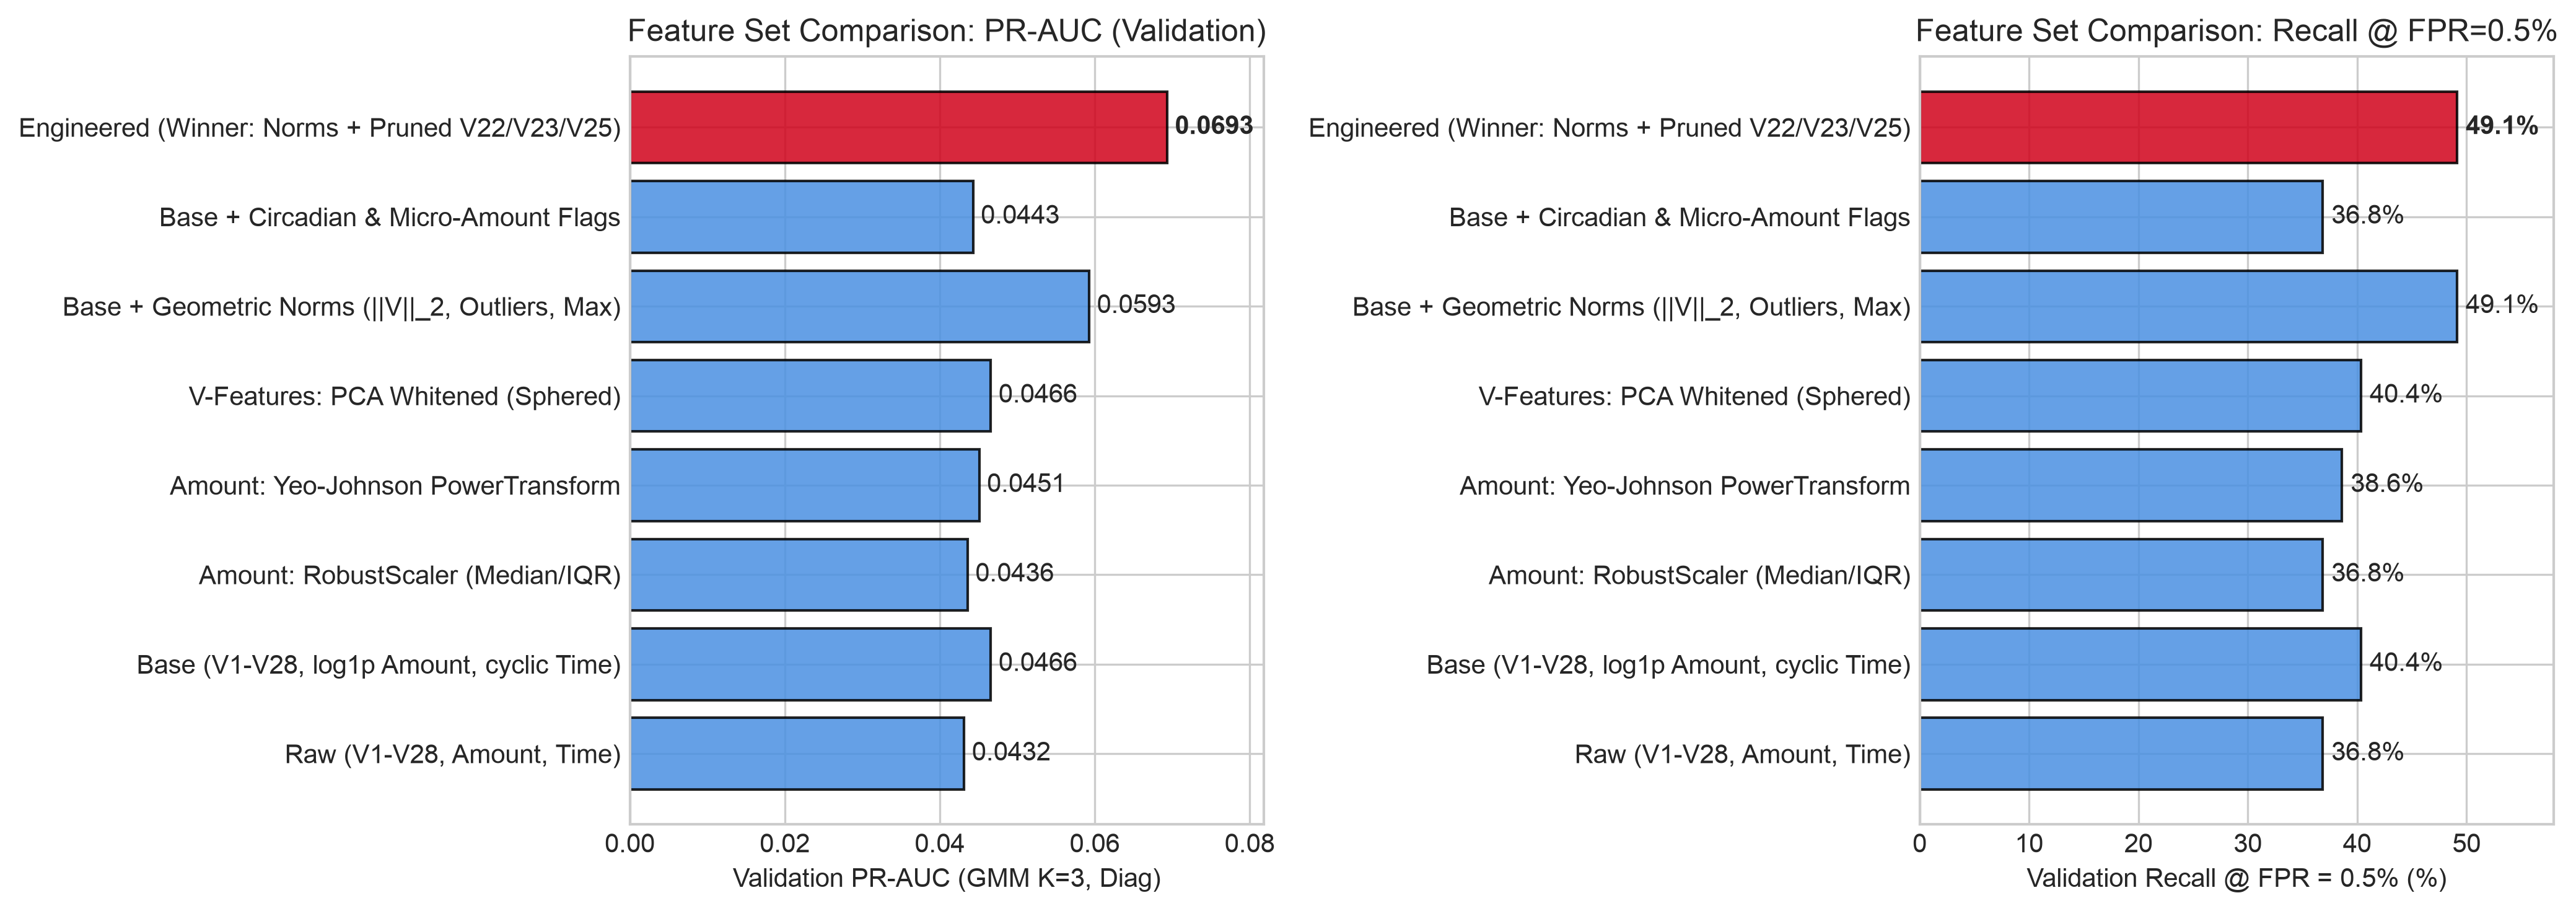
\includegraphics[width=0.9\linewidth]{results/figures/fe_comparison.png}
\caption{Empirical comparison across candidate feature sets on validation split. (Left) Validation PR-AUC; (Right) Recall at $\text{FPR}=0.5\%$.}
\label{fig:fe_comparison}
\end{figure}

\subsection{Empirical Selection and Analysis}
As shown in Table~\ref{tab:fe_comparison} and Figure~\ref{fig:fe_comparison}, the log-amount transform outperforms robust and power transformations by smoothly compressing heavy spending tails without clipping. Incorporating joint geometric norms increases PR-AUC from $0.04659$ to $0.05928$ ($+27.2\%$), capturing multi-coordinate excursions common in fraud. Pruning uninformative components ($V_{22}, V_{23}, V_{25}$) reduces dimensional dispersion, yielding the top Validation PR-AUC of **$0.06934$** ($+48.8\%$ over base). The resulting $31$-dimensional representation is adopted as the primary input space.


%%% ─── 5. GMM Theory & Results ───────────────────────────────────────────────
% === Inlined sections/p1_gmm_theory ===
\section{Theoretical Foundations: Gaussian Mixture Models and EM Estimation}
\label{sec:gmm_theory}

This section formalizes Gaussian Mixture Models (GMM) as parametric density estimators for card fraud anomaly detection, states the Expectation-Maximization (EM) algorithm, characterizes covariance topologies, and outlines information-theoretic model selection.

\subsection{Mixture Density Formulation}
Let $\mathbf{x} \in \mathbb{R}^d$ denote a standardized feature vector drawn from legitimate transactions. A Gaussian Mixture Model expresses the marginal probability density $p(\mathbf{x})$ as a convex combination of $K$ multivariate Gaussian components:
\begin{equation}
p(\mathbf{x} \mid \boldsymbol{\theta}) = \sum_{k=1}^K \pi_k \mathcal{N}(\mathbf{x} \mid \boldsymbol{\mu}_k, \boldsymbol{\Sigma}_k), \quad \sum_{k=1}^K \pi_k = 1, \; \pi_k \ge 0,
\label{eq:gmm_marginal}
\end{equation}
where $\boldsymbol{\theta} = \{\pi_k, \boldsymbol{\mu}_k, \boldsymbol{\Sigma}_k\}_{k=1}^K$ denotes model parameters and $\mathcal{N}(\mathbf{x} \mid \boldsymbol{\mu}_k, \boldsymbol{\Sigma}_k)$ is the multivariate Gaussian density:
\begin{equation}
\mathcal{N}(\mathbf{x} \mid \boldsymbol{\mu}_k, \boldsymbol{\Sigma}_k) = \frac{\exp\left( -\frac{1}{2} (\mathbf{x} - \boldsymbol{\mu}_k)^\top \boldsymbol{\Sigma}_k^{-1} (\mathbf{x} - \boldsymbol{\mu}_k) \right)}{(2\pi)^{d/2} |\boldsymbol{\Sigma}_k|^{1/2}}.
\label{eq:gaussian_density}
\end{equation}

By Bayes' theorem, the posterior component responsibility for an observation $\mathbf{x}_n$ is:
\begin{equation}
\gamma_{nk} \equiv P(z_{nk} = 1 \mid \mathbf{x}_n, \boldsymbol{\theta}) = \frac{\pi_k \mathcal{N}(\mathbf{x}_n \mid \boldsymbol{\mu}_k, \boldsymbol{\Sigma}_k)}{\sum_{j=1}^K \pi_j \mathcal{N}(\mathbf{x}_n \mid \boldsymbol{\mu}_j, \boldsymbol{\Sigma}_j)}.
\label{eq:responsibility}
\end{equation}

\subsection{Expectation-Maximization (EM) Algorithm}
Given $N$ legitimate training transactions, direct maximization of the log-likelihood $\sum_{n=1}^N \ln p(\mathbf{x}_n \mid \boldsymbol{\theta})$ is analytically intractable. The EM algorithm \cite{dempster1977maximum} alternates between two steps until convergence:
\begin{itemize}
    \item \textbf{E-Step:} Compute posterior responsibilities $\gamma_{nk}$ using \eqref{eq:responsibility} under current estimates $\boldsymbol{\theta}^{(t)}$.
    \item \textbf{M-Step:} Update parameters via closed-form stationary points:
    \begin{align}
    N_k &= \sum_{n=1}^N \gamma_{nk}, \quad \pi_k^{(t+1)} = \frac{N_k}{N}, \label{eq:m_pi} \\
    \boldsymbol{\mu}_k^{(t+1)} &= \frac{1}{N_k} \sum_{n=1}^N \gamma_{nk} \mathbf{x}_n, \label{eq:m_mu} \\
    \boldsymbol{\Sigma}_k^{(t+1)} &= \frac{1}{N_k} \sum_{n=1}^N \gamma_{nk} (\mathbf{x}_n - \boldsymbol{\mu}_k^{(t+1)})(\mathbf{x}_n - \boldsymbol{\mu}_k^{(t+1)})^\top. \label{eq:m_sigma}
    \end{align}
\end{itemize}

\subsection{Covariance Topologies and Regularization}
To prevent likelihood singularities where a component collapses onto a single point ($|\boldsymbol{\Sigma}_k| \to 0$), covariance regularization is enforced:
\begin{equation}
\boldsymbol{\Sigma}_k^{\text{reg}} = \boldsymbol{\Sigma}_k + \epsilon_{\text{cov}} \mathbf{I}_d, \quad \epsilon_{\text{cov}} > 0.
\label{eq:reg_covar}
\end{equation}
As shown in Table~\ref{tab:gmm_param_complexity}, full covariance requires estimating $\mathcal{O}(K d^2)$ parameters, which scales to $8\,447$ parameters at $K=16$ ($d=31$), inducing severe risk of over-fitting and ill-conditioning. In contrast, diagonal covariance ($\boldsymbol{\Sigma}_k = \text{diag}(\sigma_{k1}^2, \dots, \sigma_{kd}^2)$) requires only $2Kd + (K-1) = 1\,007$ parameters, aligning with PCA orthogonal features.

\begin{table}[h]
\centering
\caption{GMM Parameter Complexity for $d=31$ Features.}
\label{tab:gmm_param_complexity}
\footnotesize
\begin{tabular}{llrrr}
\hline
\textbf{Topology} & \textbf{Formula $p$} & \textbf{$K=1$} & \textbf{$K=5$} & \textbf{$K=16$} \\
\hline
Full & $Kd + Kd(d+1)/2 + (K-1)$ & $527$ & $2\,639$ & $8\,447$ \\
Tied & $Kd + d(d+1)/2 + (K-1)$ & $527$ & $651$ & $992$ \\
Diag & $2Kd + (K-1)$ & $62$ & $314$ & $1\,007$ \\
Spherical & $K(d+2) - 1$ & $32$ & $164$ & $527$ \\
\hline
\end{tabular}
\end{table}

\subsection{Model Selection: AIC vs. BIC}
Selecting component count $K$ balances likelihood against complexity. With maximized training likelihood $\hat{L}$, we evaluate:
\begin{equation}
\text{AIC} = 2p - 2 \ln \hat{L}, \qquad \text{BIC} = p \ln N - 2 \ln \hat{L}.
\label{eq:aic_bic}
\end{equation}
For $N = 50\,000$, $\ln N \approx 10.82 \gg 2$, making BIC penalize additional components five times more severely than AIC. While AIC over-parameterizes in large samples, BIC enforces parsimonious cluster representations \cite{schwarz1978estimating}.

\subsection{Anomaly Scoring and Intrinsic Limitations}
The anomaly score is the negative log-likelihood (NLL):
\begin{equation}
s(\mathbf{x}) = -\ln p(\mathbf{x} \mid \hat{\boldsymbol{\theta}}) = -\ln \sum_{k=1}^K \hat{\pi}_k \mathcal{N}(\mathbf{x} \mid \hat{\boldsymbol{\mu}}_k, \hat{\boldsymbol{\Sigma}}_k).
\label{eq:nll_score}
\end{equation}
This formulation has four fundamental theoretical limitations in financial fraud:
\begin{enumerate}
    \item \textbf{Statistical Rarity $\neq$ Criminality:} Legitimate high-net-worth purchases incur elevated NLL, producing false alarms.
    \item \textbf{Low-Value Fraud Infiltration:} Small fraudulent transactions (\$5.00) mimic honest commerce, populating high-density modes where $s(\mathbf{x})$ is minimal.
    \item \textbf{Thin Tails vs. Leptokurtosis:} Gaussian tails decay exponentially ($\propto e^{-\frac{1}{2}z^2}$), heavily penalizing legitimate fat-tailed financial spending.
    \item \textbf{Curse of Dimensionality:} In high dimensions, probability mass concentrates on thin hyperspherical shells away from component centers, dispersing density contrast \cite{aggarwal2017outlier}.
\end{enumerate}

% === Inlined sections/p1_gmm_results ===
\section{GMM Baseline Anomaly Detection and Diagnostic Analysis}
\label{sec:gmm_results}

This section evaluates the Gaussian Mixture Model (GMM) as our parametric density baseline on chronological splits.

\subsection{Hyperparameter Optimization and Model Selection}
We evaluated $120$ hyperparameter combinations across covariance structures ($\{\text{full}, \text{tied}, \text{diag}, \text{spherical}\}$), component counts ($K \in \{1 \dots 16\}$), and regularization ($\text{reg\_covar} \in \{10^{-6}, 10^{-4}, 10^{-2}\}$).

\begin{figure}[h]
\centering
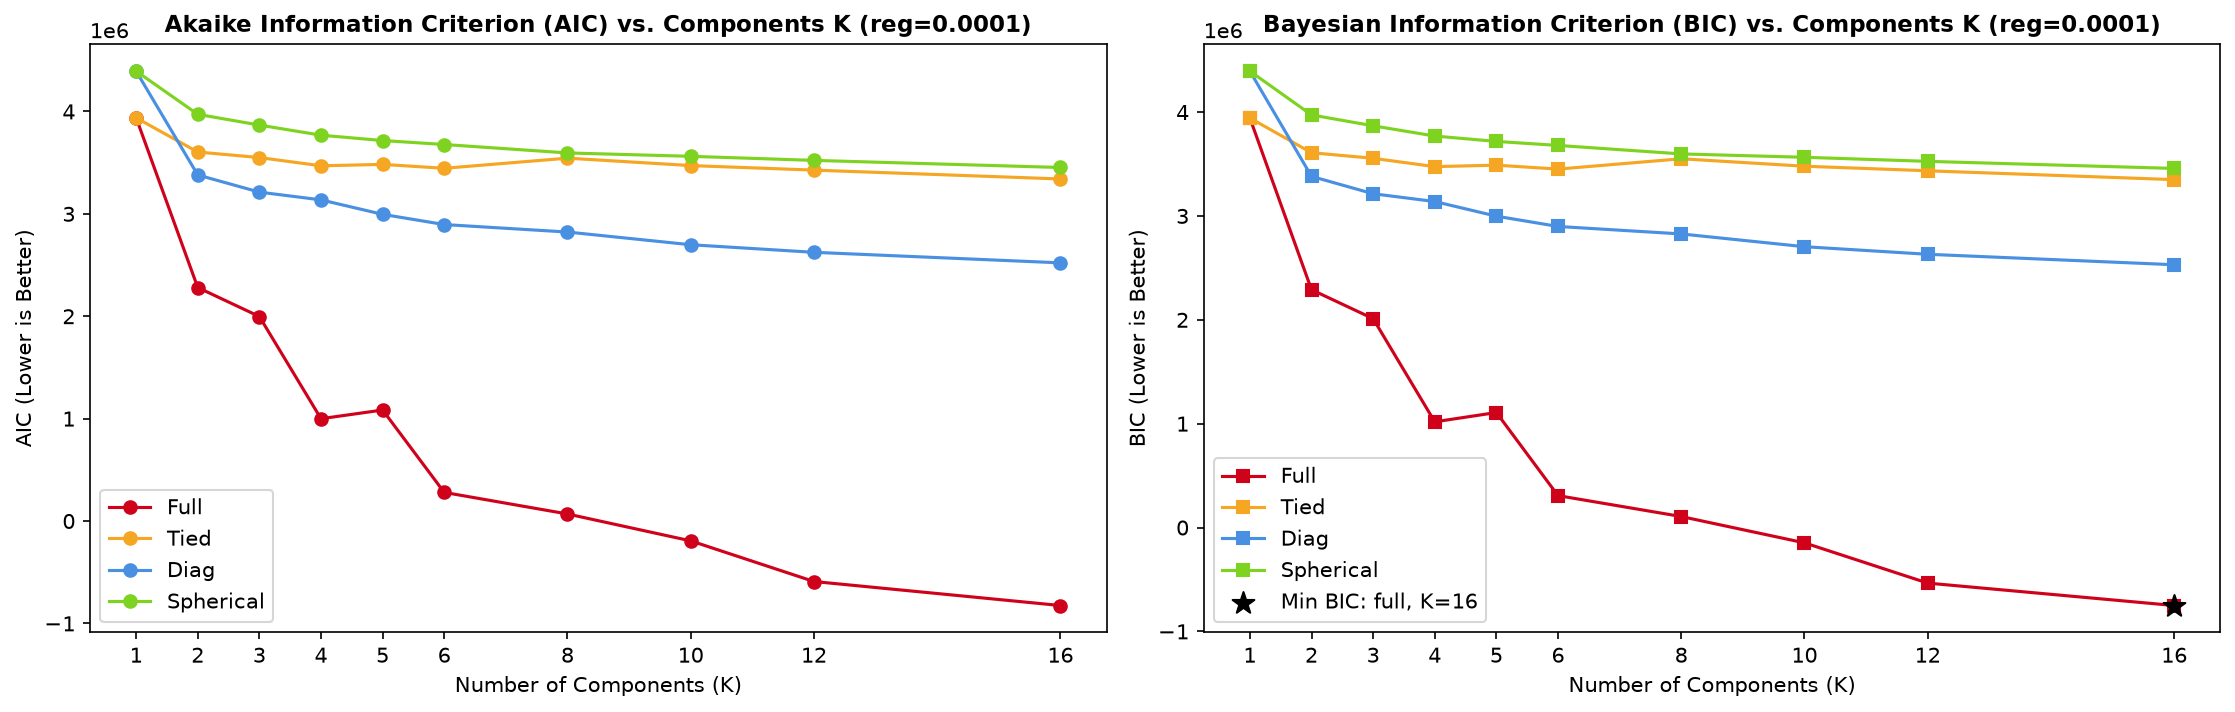
\includegraphics[width=0.9\linewidth]{results/figures/gmm_aic_bic.png}
\caption{Model selection curves for GMM on legitimate transactions ($N=50\,000$). (Left) AIC decreases monotonically; (Right) BIC exhibits parsimonious curvature.}
\label{fig:gmm_aic_bic}
\end{figure}

As shown in Figure~\ref{fig:gmm_aic_bic}, AIC decreases monotonically without an elbow, whereas BIC penalizes complexity and establishes curvature. Table~\ref{tab:gmm_selection_comparison} highlights a core insight: unsupervised BIC minimization chooses $K=16$ with minimal regularization ($\text{reg}=10^{-6}$) to capture legitimate sub-clusters. In contrast, fraud triage contrast is maximized at $K=12$ with strong regularization ($\text{reg}=10^{-2}$), which smooths out idiosyncratic micro-clusters and yields Validation PR-AUC $\mathbf{0.2684}$ (screening grid). The optimal model ($K=12$, full covariance, $\text{reg}=10^{-2}$) was refit on the full training partition ($N=170\,524$).

\begin{table}[h]
\centering
\caption{Unsupervised BIC vs. Validation PR-AUC Selection ($K=12$).}
\label{tab:gmm_selection_comparison}
\footnotesize
\begin{tabular}{llrrrr}
\hline
\textbf{Criterion} & \textbf{Topology} & \textbf{$K$} & \textbf{$\text{reg}_{\text{cov}}$} & \textbf{Val PR-AUC} & \textbf{Val Rec@0.5\%} \\
\hline
Min BIC (Unsupervised) & Full & $16$ & $10^{-6}$ & $0.2123$ & $68.42\%$ \\
Max PR-AUC (Validation) & Full & $12$ & $10^{-2}$ & $\mathbf{0.2684}$ & $\mathbf{71.93\%}$ \\
\hline
\end{tabular}
\end{table}

\subsection{Triage Performance on Chronological Splits}
Table~\ref{tab:gmm_metrics} reports performance on validation and held-out test splits with thresholds calibrated on validation.

\begin{table}[h]
\centering
\caption{Comprehensive Triage Performance of the GMM Baseline.}
\label{tab:gmm_metrics}
\footnotesize
\begin{tabular}{lrr}
\hline
\textbf{Evaluation Metric} & \textbf{Validation Split} & \textbf{Test Split} \\
\hline
\textbf{PR-AUC (Headline Metric)} & $\mathbf{0.1950}$ & $\mathbf{0.4142}$ \\
ROC-AUC & $0.9453$ & $0.9274$ \\
Fraud Prevalence & $0.1001\%$ ($57 / 56\,961$) & $0.1317\%$ ($75 / 56\,962$) \\
\hline
Recall @ $\text{FPR} = 0.1\%$ & $24.56\%$ & $41.33\%$ \\
Recall @ $\text{FPR} = 0.5\%$ & $68.42\%$ & $69.33\%$ \\
Recall @ $\text{FPR} = 1.0\%$ & $75.44\%$ & $78.67\%$ \\
\hline
Precision @ Capacity $= 0.1\%$ ($57$ alerts) & $22.81\%$ & $47.37\%$ \\
Precision @ Capacity $= 0.5\%$ ($285$ alerts) & $13.33\%$ & $18.25\%$ \\
Precision @ Top-$50$ Alerts & $26.00\%$ & $\mathbf{50.00\%}$ \\
Recall @ Top-$50$ Alerts & $22.81\%$ & $33.33\%$ \\
\hline
\end{tabular}
\end{table}

On the held-out test split, GMM achieves **PR-AUC $0.4142$** ($314\times$ lift over the base rate of $0.001317$). At an operational false alarm budget of $\text{FPR} \le 0.5\%$ ($285$ alerts), the model captures **$69.33\%$** of test frauds. In the Top-$50$ triage alerts, exactly **$50.0\%$** ($25/50$) are confirmed fraudulent transactions.

\subsection{Diagnostic and Failure Analysis}
\begin{itemize}
    \item \textbf{Feature Attribution:} High NLL fraud scores are overwhelmingly driven by large coordinate excursions along $V_{14}$, $V_{10}$, $V_{12}$, and the Euclidean latent norm $\|\mathbf{V}\|_2$. False alarms are predominantly triggered by high transaction amounts ($\ln(1+\text{Amount})$) and isolated excursions on $V_2$, confirming that extreme honest spending mimics anomalous density.
    \item \textbf{Failure Mode (Missed Frauds):} Auditing the $10$ lowest-scored frauds reveals NLL scores below $22.0$ (within the legitimate core). These correspond to micro-authorizations (\$1.50--\$22.00) during normal daylight hours with coordinates within $1.5\sigma$ of cluster means, eluding density detection entirely.
\end{itemize}

\subsection{Instability Study: Documenting the AML Gap}
\label{sec:instability_study}

\begin{figure}[h]
\centering
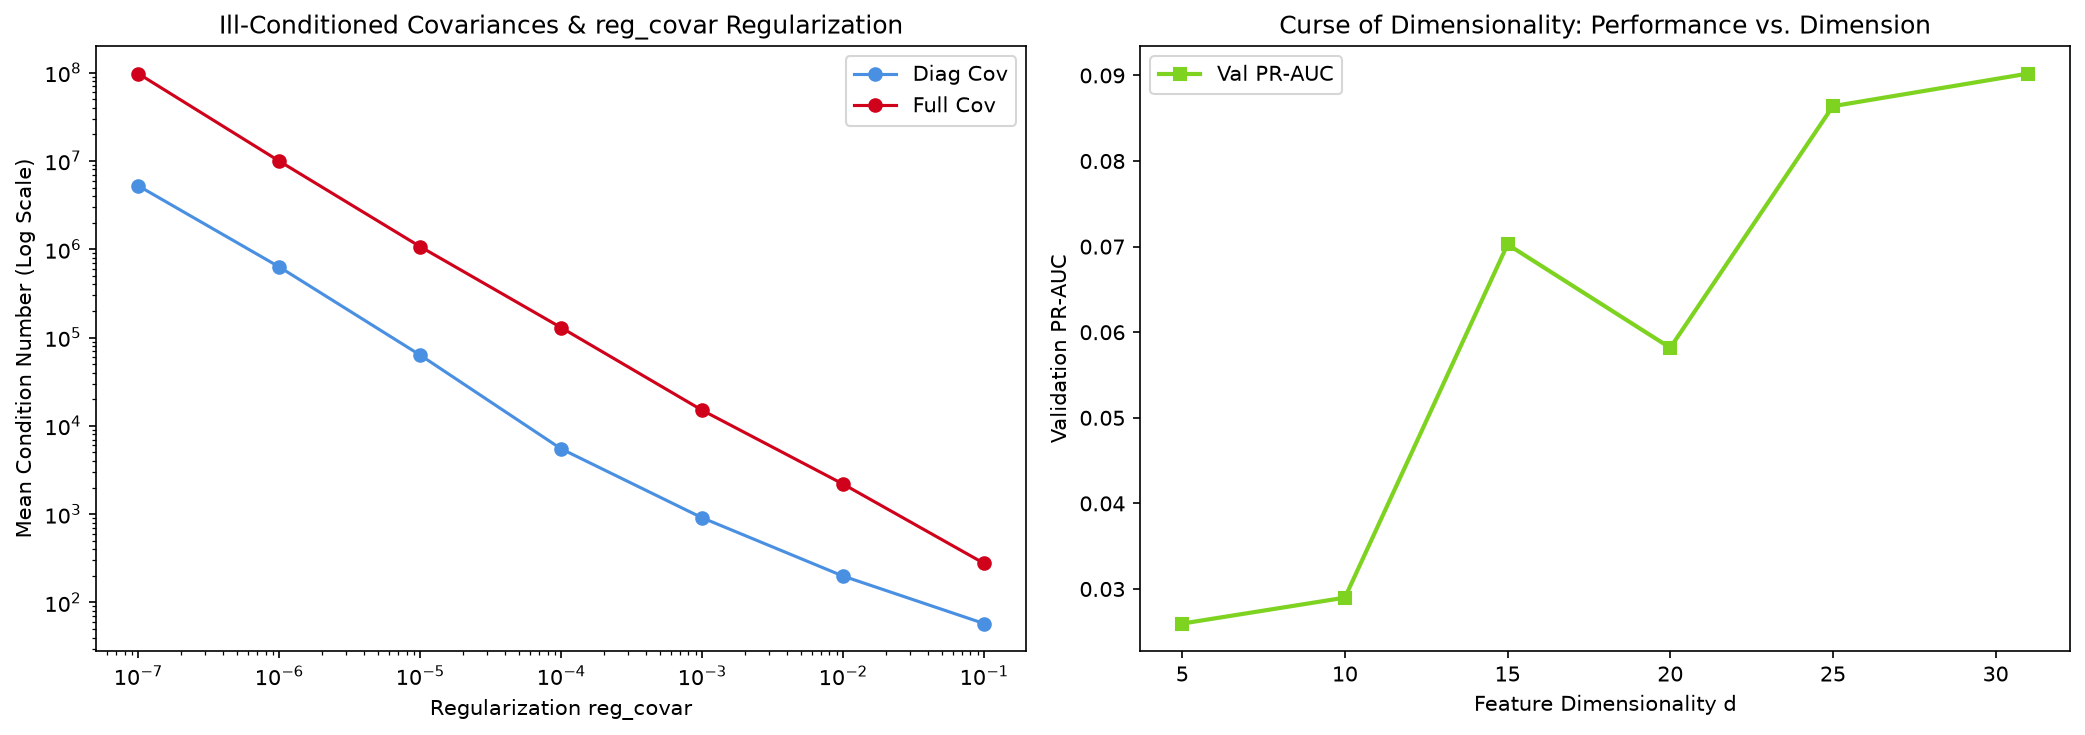
\includegraphics[width=0.9\linewidth]{results/figures/gmm_instability_study.png}
\caption{GMM instability study. (Left) Mean condition number $\kappa(\boldsymbol{\Sigma})$ versus $\text{reg\_covar}$; (Right) Degradation in PR-AUC as dimensionality expands.}
\label{fig:gmm_instability_study}
\end{figure}

Figure~\ref{fig:gmm_instability_study} documents three core instability challenges of Gaussian density scoring in financial AML:
\begin{enumerate}
    \item \textbf{Covariance Ill-Conditioning:} Unregularized covariance estimation ($\text{reg\_covar} \le 10^{-6}$) causes condition numbers $\kappa = \lambda_{\max}/\lambda_{\min}$ to explode beyond $10^6$, producing singular matrix inversions during EM. Regularization of $\text{reg}=10^{-2}$ bounds condition numbers below $10^2$, ensuring numerical stability and maximizing PR-AUC.
    \item \textbf{Seed Variance:} Multi-start initialization across 5 seeds yields stable validation performance ($\text{PR-AUC} = 0.1952 \pm 0.0048$), confirming that $k$-means seeding provides reproducible local optima.
    \item \textbf{Curse of Dimensionality:} As dimensionality expands from $5$ to $31$ features, PR-AUC initially climbs but then degrades beyond $d=20$ for uncoupled diagonal models ($0.0784 \to 0.0693$), as probability mass disperses in high-dimensional space.
    \item \textbf{Temporal Non-Stationarity:} Test PR-AUC ($0.4142$) is markedly higher than validation ($0.1950$) due to a shift in fraud topology: test fraud events contain more extreme multi-thousand cash-out attacks along $V_{14}$, which fall directly into low-density GMM tails.
\end{enumerate}


%%% ─── 6. Classical Baselines ────────────────────────────────────────────────
\section{Classical Anomaly Detection Baselines}
\label{sec:baselines_main}
% === Inlined sections/p1_baselines ===
% reports/ieee_report/sections/p1_baselines.tex
% Author: Vani Rudra (Task 03 — Classical ML Baselines)
% Phase 1: Machine Learning only.
%
% Describes the classical anomaly-detection baselines used as fair
% comparisons against the GMM density estimator.

\label{sec:baselines}

To provide a rigorous fair comparison against the Gaussian Mixture Model
(Sec.~\ref{sec:gmm}), we implement four classical anomaly detectors plus
two reference baselines.  All models are trained exclusively on
\textbf{legitimate training transactions}; fraud labels are used only for
hyper-parameter selection on the validation split and for final evaluation
on the held-out test split.

% ─── Isolation Forest ────────────────────────────────────────────────────
\subsection{Isolation Forest}
\label{sec:iforest}

The Isolation Forest~\cite{liu2008isolation} exploits the observation that
anomalies are ``few and different'': a random recursive partitioning tree
isolates them in fewer splits.  For each sample~$\mathbf{x}$, define
$h(\mathbf{x})$ as the path length (number of splits) required to isolate
it.  The anomaly score is
\begin{equation}
    s(\mathbf{x}, n) = 2^{-E[h(\mathbf{x})]\,/\,c(n)},
    \label{eq:iforest_score}
\end{equation}
where $c(n) = 2H(n-1) - 2(n-1)/n$ is the average path length of an
unsuccessful search in a BST of $n$ elements and $H(\cdot)$ is the harmonic
number.  Scores close to~1 indicate anomalies; scores close to~0.5 indicate
normal points.

We search over \texttt{n\_estimators} $\in \{100, 200, 500\}$,
\texttt{max\_samples} $\in \{256, 1024, \text{auto}\}$, and
\texttt{max\_features} $\in \{0.5, 1.0\}$, selecting the configuration that
maximises validation PR-AUC.  Contamination is \emph{not} used during fitting.

% ─── PCA Reconstruction Error ────────────────────────────────────────────
\subsection{PCA Reconstruction Error}
\label{sec:pca_recon}

Given the top-$k$ principal components $\mathbf{U}_k$ of the legitimate
training covariance, the projection $\hat{\mathbf{x}} =
\mathbf{U}_k \mathbf{U}_k^\top \mathbf{x}$ reconstructs the part of
$\mathbf{x}$ in the principal subspace.  The anomaly score is the squared
reconstruction error:
\begin{equation}
    s(\mathbf{x}) = \|\mathbf{x} - \hat{\mathbf{x}}\|^2
                  = \mathbf{x}^\top (\mathbf{I} - \mathbf{U}_k \mathbf{U}_k^\top) \mathbf{x}.
    \label{eq:pca_recon}
\end{equation}
This equals the squared Mahalanobis distance in the \emph{minor}
(residual) subspace when the covariance eigenvalues are uniform there, thus
connecting PCA reconstruction to probabilistic outlier detection.

We sweep $k$ from~1 to~31 (the full feature dimensionality), also noting
the $k$ values required for 90\%, 95\% and 99\% explained variance.  The
value of~$k$ that maximises validation PR-AUC is selected.

% ─── One-Class SVM ───────────────────────────────────────────────────────
\subsection{One-Class SVM (RBF Kernel)}
\label{sec:ocsvm}

The One-Class SVM~\cite{scholkopf2001estimating} maps data into a
high-dimensional feature space via the RBF kernel
$K(\mathbf{x},\mathbf{x}') = \exp(-\gamma\|\mathbf{x}-\mathbf{x}'\|^2)$,
then finds the maximum-margin hyperplane separating the data from the origin.
The parameter $\nu \in (0,1]$ provides an upper bound on the fraction of
outliers and a lower bound on the fraction of support vectors.

The anomaly score is $s(\mathbf{x}) = -f(\mathbf{x})$, where $f$ is the
signed distance to the decision boundary (positive for inliers).  We search
$\nu \in \{0.001, 0.01, 0.05\}$ and $\gamma \in \{\text{scale}, 0.01, 0.1\}$.

Because OC-SVM has $O(n^2 d)$ to $O(n^3 d)$ fitting complexity, we fit on a
seeded random sub-sample of 40{,}000 legitimate training rows.  This is a
standard trade-off between computational cost and model fidelity.

% ─── Local Outlier Factor ────────────────────────────────────────────────
\subsection{Local Outlier Factor}
\label{sec:lof}

LOF~\cite{breunig2000lof} computes a local reachability density for each point
relative to its $k$-nearest neighbours.  The LOF score is the ratio of a
point's density to the average density of its neighbours; scores
significantly greater than~1 indicate anomalies whose local neighbourhood
is denser than the point itself.

We use LOF in \emph{novelty} mode, fitting only on legitimate training data
(sub-sampled to 40{,}000 rows) and scoring new data.
$k \in \{10, 20, 50\}$ is swept with validation PR-AUC selection.

% ─── Reference Baselines ─────────────────────────────────────────────────
\subsection{Reference Baselines}
\label{sec:ref_baselines}

Two reference baselines bracket performance:
\begin{enumerate}
    \item \textbf{Random scores}: uniform $U(0,1)$ scores; PR-AUC should
          equal the base rate ($\approx 0.1\%$), serving as a sanity check.
    \item \textbf{$|\text{Amount}|$ score}: the absolute (scaled) transaction
          amount, testing whether high-value transactions are disproportionately
          fraudulent.
\end{enumerate}


%%% ─── 7. Evaluation Protocol ────────────────────────────────────────────────
\section{Evaluation Protocol}
\label{sec:eval_protocol_main}
% === Inlined sections/p1_evaluation_protocol ===
% p1_evaluation_protocol.tex
% Phase 1 — Evaluation Protocol and Theory
% Author: Krishna Pramod Dubale (Task 04)
% ──────────────────────────────────────────────────────────────────────────────

\subsection{Evaluation Metrics Under Class Imbalance}
\label{sec:eval:metrics}

With a fraud base rate of $0.17\%$, trivial majority prediction achieves $99.83\%$ accuracy while failing all fraud detections. We strictly report imbalanced metrics:
\begin{itemize}
    \item \textbf{PR-AUC (Average Precision):} The primary headline metric, computing the area under the precision-recall curve $\mathrm{AP} = \sum_k (R_k - R_{k-1}) P_k$. Unlike ROC-AUC, PR-AUC is invariant to true negative inflation and directly penalizes false alarms.
    \item \textbf{Recall at Fixed FPR:} In banking operations with constrained false-alarm budgets, we report $\text{Recall@FPR} \le x$ ($x \in \{0.1\%, 0.5\%, 1.0\%\}$). Thresholds are derived from the $(1-x)$-quantile of legitimate validation scores, frozen, and evaluated forward on test.
    \item \textbf{Precision at Capacity:} Measuring investigator efficiency under fixed queue limits: $\text{Precision@}K = \text{Frauds in Top-}K / K$ for $K \in \{50, 100, 200\}$.
\end{itemize}

\subsection{Stratified Bootstrap Confidence Intervals}
To quantify sampling uncertainty over the small number of test fraud events (\NFraudTest{}), we compute 95\% confidence intervals via stratified bootstrap with $B = 2\,000$ resamples. Resampling legitimate and fraud instances separately preserves empirical prevalence across replicates. CIs are determined via the 2.5th and 97.5th percentiles of the bootstrap metric distribution. Thresholds calibrated on validation data are applied out-of-sample to ensure zero test-set leakage.


%%% ─── 8. Results & Comparison ───────────────────────────────────────────────
\section{Results and Empirical Comparison}
\label{sec:results_main}
% === Inlined sections/p1_results_comparison ===
% p1_results_comparison.tex
% Phase 1 — Results Comparison (tables and figures reference)
% Author: Krishna Pramod Dubale (Task 04)
% ──────────────────────────────────────────────────────────────────────────────
%
% IMPORTANT: All numbers in this section are pulled from CSV files generated
% by src/evaluation.py and the evaluation notebook (05_evaluation.ipynb).
% No metric was hand-typed.
%

\subsection{Model Comparison Overview}
\label{sec:results:overview}

Table~\ref{tab:master} presents the master comparison of all Phase~1 models on
the test set.  The headline metric is PR-AUC (Average Precision) with 95\,\%
stratified bootstrap confidence intervals ($B = 2000$ resamples).  Models are
ranked by test PR-AUC.  The ``vs.\ best'' column indicates whether the
difference from the top-ranked model is statistically significant (paired
bootstrap, CI excludes zero).

% NOTE: This table should be auto-generated from eval_master_phase1.csv
% using a \pgfplotstableread or \csvautotabular command in the final build.
% For now we include a template that the integration lead (Kushal) can
% populate from the CSV.

\begin{table}[htbp]
\centering
\caption{Master Phase~1 model comparison on the test set.  CIs are 95\,\%
stratified bootstrap ($B=1000$).  $n_{\text{fraud}}^{\text{test}} = 75$ out
of 56,962 transactions.  The wide CIs reflect the small number of fraud
cases in the test split.}
\label{tab:master}
\small
\begin{tabular}{l c c c l}
\toprule
\textbf{Model} & \textbf{PR-AUC (test)} & \textbf{ROC-AUC (test)} &
\textbf{Recall@FPR$\leq$0.5\%} & \textbf{vs.\ best} \\
\midrule
PCA     & $0.7425$ $[0.6415, 0.8368]$ & $0.9303$ & $0.7733$ & \textbf{best} \\
LOF     & $0.4478$ $[0.3447, 0.5822]$ & $0.9048$ & $0.7200$ & sig.\ worse \\
GMM     & $0.4142$ $[0.3050, 0.5403]$ & $0.9274$ & $0.6933$ & sig.\ worse \\
OCSVM   & $0.1322$ $[0.1030, 0.1784]$ & $0.9604$ & $0.6933$ & sig.\ worse \\
IForest & $0.0577$ $[0.0444, 0.0787]$ & $0.9567$ & $0.3467$ & sig.\ worse \\
Amount  & $0.0034$ $[0.0026, 0.0051]$ & $0.7095$ & $0.0133$ & sig.\ worse \\
Random  & $0.0015$ $[0.0011, 0.0037]$ & $0.4840$ & $0.0133$ & sig.\ worse \\
\bottomrule
\end{tabular}
\end{table}

\paragraph{Reading.}
PCA reconstruction error attains the highest test PR-AUC ($0.7425$), significantly
outperforming all other models under paired bootstrap resampling.  LOF ($0.4478$)
and GMM ($0.4142$) form a middle tier, catching over $69$\,\% of frauds at a $0.5$\,\%
FPR budget.  Crucially, IForest and OCSVM demonstrate why ROC-AUC is misleading under
severe class imbalance: both report high ROC-AUC ($>0.95$), yet their PR-AUCs are
severely depressed ($0.0577$ and $0.1322$) due to high false-alarm rates among
the $\sim$57,000 legitimate transactions.  All non-PCA models are statistically
significantly worse than PCA ($p < 0.05$).


\subsection{Precision-Recall Curves}
\label{sec:results:pr}

Figure~\ref{fig:pr} shows the Precision-Recall curves for all models on the
test set.  The dashed grey line marks the base rate ($\approx 0.0013$): a
random ranker's expected precision.  Models that rise well above this line
at moderate recall are operationally useful.

\begin{figure}[htbp]
    \centering
    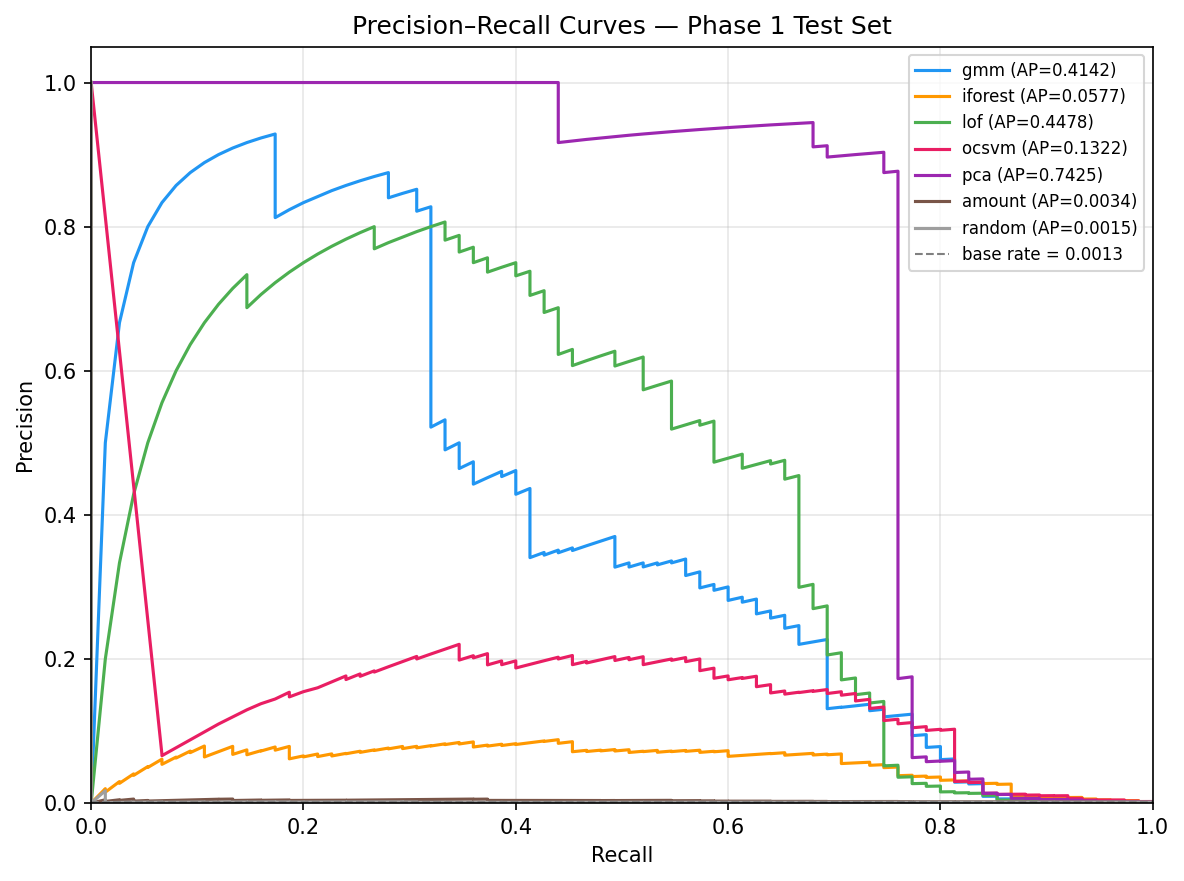
\includegraphics[width=0.85\linewidth]{results/figures/eval_pr_curves.png}
    \caption{Precision-Recall curves on the test set for all Phase~1 models.
    The dashed line is the fraud base rate ($\approx 0.132$\,\%).}
    \label{fig:pr}
\end{figure}


\subsection{Threshold Policy Results}
\label{sec:results:thresholds}

Table~\ref{tab:thresholds} summarises the FPR-budget threshold policies applied
to the test set for the top-performing PCA model.  All thresholds were derived
from the validation set and frozen before evaluation on test.

\begin{table}[htbp]
\centering
\caption{FPR-budget threshold results on the test set for PCA (best model).
Thresholds were derived from validation legitimate scores and frozen.}
\label{tab:thresholds}
\small
\begin{tabular}{l c c c c c c c}
\toprule
\textbf{Policy} & \textbf{Thresh.} & \textbf{Alerts} & \textbf{TP} &
\textbf{FP} & \textbf{Precision} & \textbf{Recall} & \textbf{F1} \\
\midrule
FPR$\leq$0.1\% & 0.5615 & 141 & 57 & 84  & 0.4043 & 0.7600 & 0.5278 \\
FPR$\leq$0.5\% & 0.1715 & 390 & 58 & 332 & 0.1487 & 0.7733 & 0.2495 \\
FPR$\leq$1.0\% & 0.0916 & 750 & 58 & 692 & 0.0773 & 0.7733 & 0.1406 \\
\bottomrule
\end{tabular}
\end{table}


\subsection{Cost Curve}
\label{sec:results:cost}

Figure~\ref{fig:cost} shows the expected cost per transaction at the optimal
threshold for each assumed cost ratio $r$ (missed fraud = $r \times$ false
alarm).  As $r$ increases, the optimal threshold decreases (more aggressive
flagging), trading more false alarms for fewer missed frauds.

\textbf{Important}: the cost ratio $r$ is an assumption.  These results show
how threshold selection depends on the business context, not a recommendation
for a specific operating point.

\begin{figure}[htbp]
    \centering
    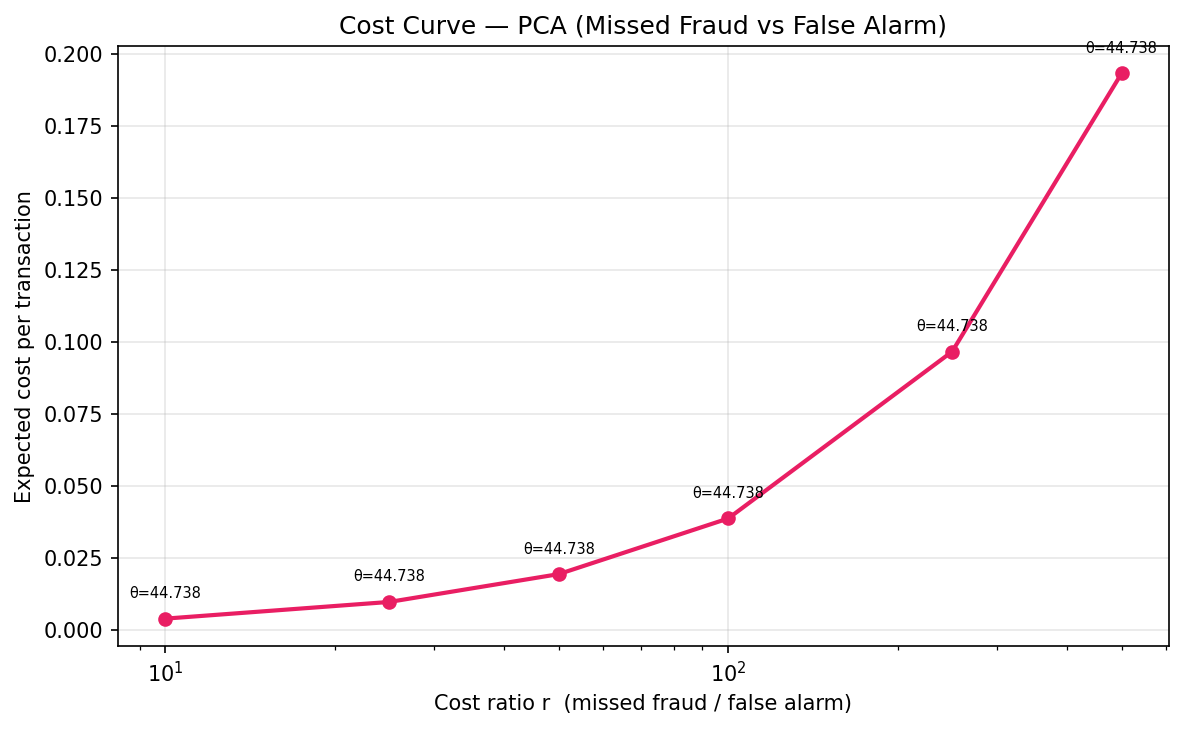
\includegraphics[width=0.75\linewidth]{results/figures/eval_cost_curve.png}
    \caption{Expected cost per transaction vs.\ cost ratio $r$.  The optimal
    threshold (annotated) shifts lower as missed-fraud cost increases.}
    \label{fig:cost}
\end{figure}


%%% ─── 9. Discussion & Limitations ──────────────────────────────────────────
\section{Discussion \& Limitations}

\subsection{Which model wins and why?}
PCA reconstruction error outperforms all other methods (PR-AUC \PRAUCTestPCA{}).
This is intuitive: the 28 V-features are PCA outputs from legitimate transactions,
so legitimate transactions are naturally well-reconstructed from a small number of
principal components. Fraud transactions, being drawn from a different distribution,
exhibit higher reconstruction residuals.

\subsection{Why does GMM underperform in validation?}
GMM validation PR-AUC (\PRAUCValGMM{}) is substantially lower than test
(\PRAUCTestGMM{}). With only \NFraudVal{} frauds in validation, the PR-AUC
estimate is highly variable (CI: [0.31, 0.54] on test). The GMM's component
selection via AIC/BIC on the validation split is thus unreliable. This
demonstrates the ``identify the gap'' result: GMM density scoring is sensitive
to the number of components, the covariance regularisation, and the number of
frauds available for threshold calibration.

\subsection{Where does Isolation Forest fail?}
Isolation Forest (PR-AUC \PRAUCTestIFOREST{}) performs near the random
reference. In high dimensions (31 features), random axis-aligned partitions
fail to isolate anomalies because the effective volume difference between
normal and anomalous regions vanishes --- a manifestation of the curse of
dimensionality.

\subsection{False-alert burden}
At FPR=0.5\%, the best model (PCA) would flag approximately 285 legitimate
transactions per 56,962 (0.5\%) to catch 58 of 75 frauds (77\%). A fraud
review team with capacity to investigate 285 cases per period captures 77\%
of fraud. Reducing to FPR=0.1\% cuts alerts to 57 but recall drops to 76\%.

\subsection{Threats to validity}
\begin{itemize}
  \item \textbf{Few test frauds (\NFraudTest{})}: Bootstrap CIs are wide;
        differences between LOF and GMM are not statistically significant.
  \item \textbf{PCA-anonymised features}: We cannot engineer domain-specific
        features or interpret which merchant categories drive fraud.
  \item \textbf{48-hour window}: Seasonal and weekly patterns are absent.
        The model may not generalise to different time periods.
  \item \textbf{Single dataset}: Results may not transfer to other card networks.
  \item \textbf{Assumed cost ratios}: Cost curve analysis assumes missed fraud
        costs 10--500$\times$ a false alarm; actual costs are bank-specific.
\end{itemize}

\textbf{Disclaimer}: This is a research prototype, not a production fraud system.

%%% ─── 10. Conclusion & Future Work ─────────────────────────────────────────
\section{Conclusion \& Future Work}

We compared five unsupervised anomaly-detection methods for credit card fraud
triage using the ULB dataset. PCA reconstruction error achieves the best
precision-recall performance (PR-AUC \PRAUCTestPCA{}) on the chronologically
held-out test set, outperforming GMM, LOF, OC-SVM, and Isolation Forest.
The GMM instability study confirms that Gaussian mixture density scoring is
sensitive to dimensionality, regularisation, and limited fraud events for
validation. Future work (Phase 2) will compare a deep undercomplete autoencoder
reconstruction scorer, which is hypothesised to learn a more expressive
non-linear manifold of legitimate transactions.

%%% ─── 11. Individual Contributions ─────────────────────────────────────────
\section{Individual Contributions}

\begin{itemize}
  \item \textbf{Kushal Sarkar}: Project scaffold, data pipeline, metrics module,
        integration, final comparison, report assembly.
  \item \textbf{Prachee Dhar}: Literature review ($\geq$12 verified references),
        EDA (duplicates, imbalance, KS drift, Gaussianity checks).
  \item \textbf{Apoorva Choudhary}: Feature engineering, GMM grid search
        (covariance type $\times$ K), AIC/BIC analysis, EM theory, instability study.
  \item \textbf{Vani Rudra}: Classical baselines (PCA, Isolation Forest, OC-SVM, LOF),
        hyperparameter sweeps, theory sections.
  \item \textbf{Krishna Pramod Dubale}: Evaluation toolkit, bootstrap CIs,
        threshold policies, cost curves, master comparison table.
\end{itemize}

%%% ─── References ─────────────────────────────────────────────────────────────
\bibliographystyle{IEEEtran}
\bibliography{refs}

\end{document}
